\begin{figure}[htbp]
\centering
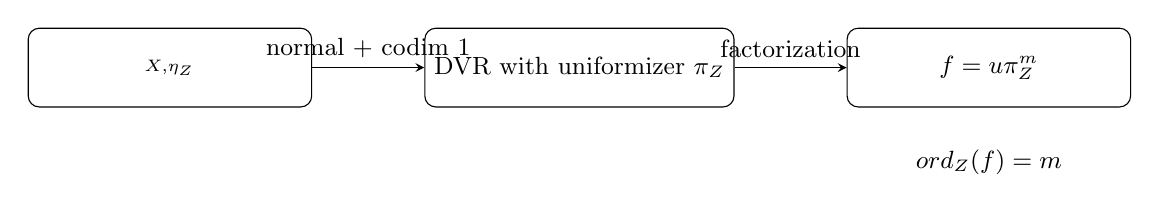
\begin{tikzpicture}[>=stealth, every node/.style={font=\small}]
\node[draw,rounded corners,minimum width=3.6cm,minimum height=1cm] (a) at (0,0) {$\OO_{X,\eta_Z}$};
\node[draw,rounded corners,minimum width=3.6cm,minimum height=1cm] (b) at (5.2,0) {DVR with uniformizer $\pi_Z$};
\node[draw,rounded corners,minimum width=3.6cm,minimum height=1cm] (c) at (10.4,0) {$f=u\pi_Z^m$};
\draw[->] (a) -- node[above]{normal + codim $1$} (b);
\draw[->] (b) -- node[above]{factorization} (c);
\node at (10.4,-1.2) {$\operatorname{ord}_Z(f)=m$};
\end{tikzpicture}
\caption{Normality turns codimension-one local algebra into a discrete valuation.}
\label{fig:vi39-dvr}
\end{figure}